\label{subsec:partycjonowanie}
Patrycjonowanie to proces zmiany układu partycji na dysku twardym. Jest to najważniejszy etap instalacji systemu gdyż to od niego w dużej mierze zależy jak system będzie działał. Pamiętaj, że na tym etapie pracujesz na danych zapisanych na dysku twardym. Chwila nieuwagi może spowodować utratę jego zawartości.

\subsubsection{Czysty dysk - wykorzystanie całego dostępnego miejsca}
\begin{center}
	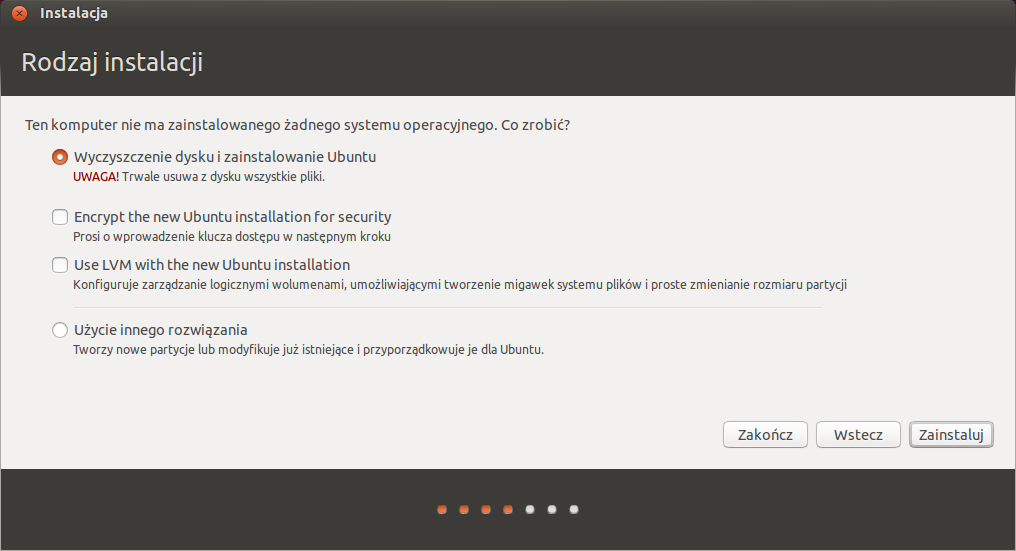
\includegraphics[scale=0.5]{images/instalator_partycjonowanie_proste.png}]
\end{center}

Jeżeli na dysku twardym nie ma żadnego innego systemu operacyjnego, instalator ubuntu zaproponuje wykorzystanie całej dostępnej przestrzeni. Instalator sam dobierze odpowiedni rozmiar partycji systemowej, partycji wymiany oraz partycji użytkownika.
\begin{flushright}
Kliknij na przycisk \textbf{Zainstaluj} aby przejść dalej.\\
Zostaniesz poproszony o potwierdzenie. Upewnij się, że wszystko jest w pożądku i kliknij \textbf{Naprzód}.\\
W tym momencie wybrane zmiany zostaną zapisane na dysku twardym.
\end{flushright}
\clearpage

\subsubsection{Instalacja przy zainstalowanym Ubuntu}
\begin{center}
	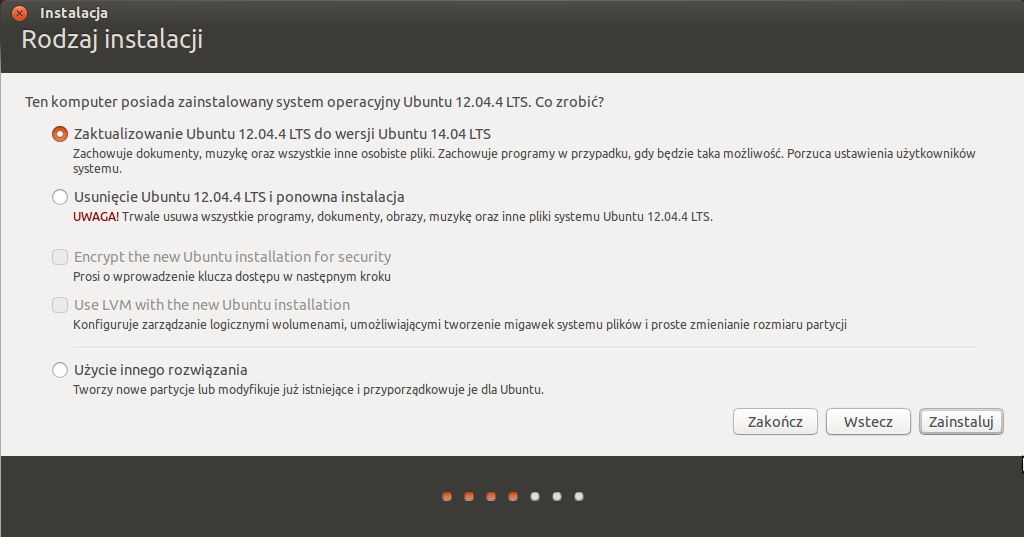
\includegraphics[scale=0.5]{images/instalator_partycjonowanie_obok_ubuntu.png}]
\end{center}
Jeżeli instalator wykryje obecność wcześniej zainstalowanej innej wersji Ubuntu to zaproponuje kilka innych rozwiązań.

Po pierwsze zaproponuje aktualizację zainstalowanego systemu do najnowszego wydania. Wszystkie dane w katalogu domowym użytkownika zostaną zachowane: muzyka, filmy, dokumenty, pliki na pulpicie, osobieste ustaienia programów, zakładki i historia przeglądarki itp.
Skasowane zostaną zainstalowane w systemie programy oraz ustawienia systemowe. Instalator zaktualizuje istniejące na dysku oprogramowanie i ewentualnie pobierze aktualizacje z internetu (jeżeli wybrałeś wcześniej tą opcję).

Drugą opcją jest usunięcie zainstalowanego Ubuntu i ponowna instalacja systemu. Wszystkie dane zostaną wymazane.
\begin{flushright}
Kliknij na przycisk \textbf{Zainstaluj} aby przejść dalej.\\
Zostaniesz poproszony o potwierdzenie. Upewnij się, że wszystko jest w pożądku i kliknij \textbf{Naprzód}.\\
W tym momencie wybrane zmiany zostaną zapisane na dysku twardym.
\end{flushright}
\clearpage

\subsubsection{Instalacja obok Windowsa}
\begin{center}
	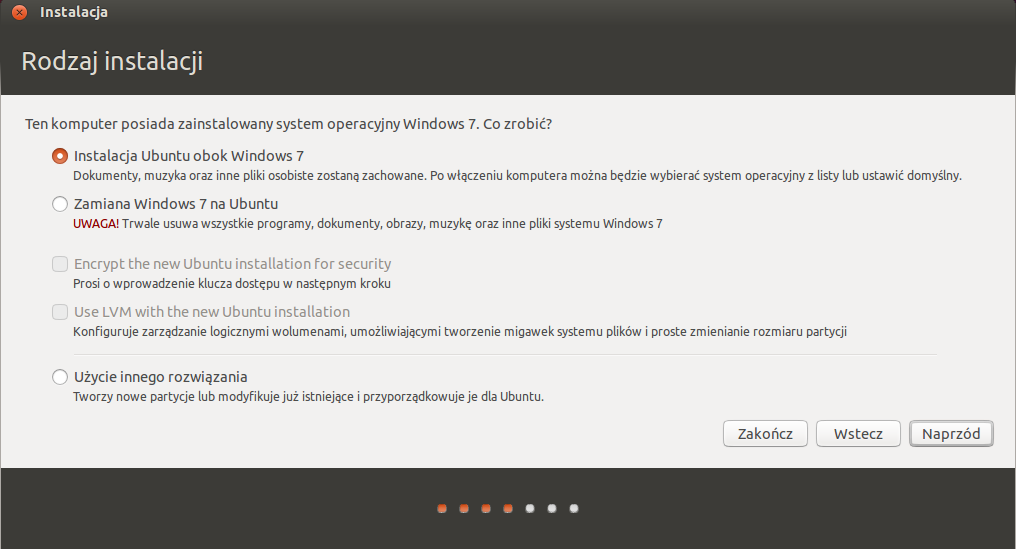
\includegraphics[scale=0.5]{images/instalator_partycjonowanie_obok_wondows7.png}]
\end{center}
Jeżeli instalator wykryje obecnosć wcześniej zainstalowanego systemu Windows to zaproponuje inne rozwiązanie. Opcja "Zamiana Windows na Ubuntu" wymaże całą zawartość partycji Windows (wraz ze wszystkimi danymi) i zamiast tego zainstaluje Ubuntu. Zostało to opisane dwie strony wcześniej.
\begin{flushright}
Kliknij na przycisk \textbf{Zainstaluj} aby przejść dalej.
\end{flushright}
\clearpage
\begin{center}
	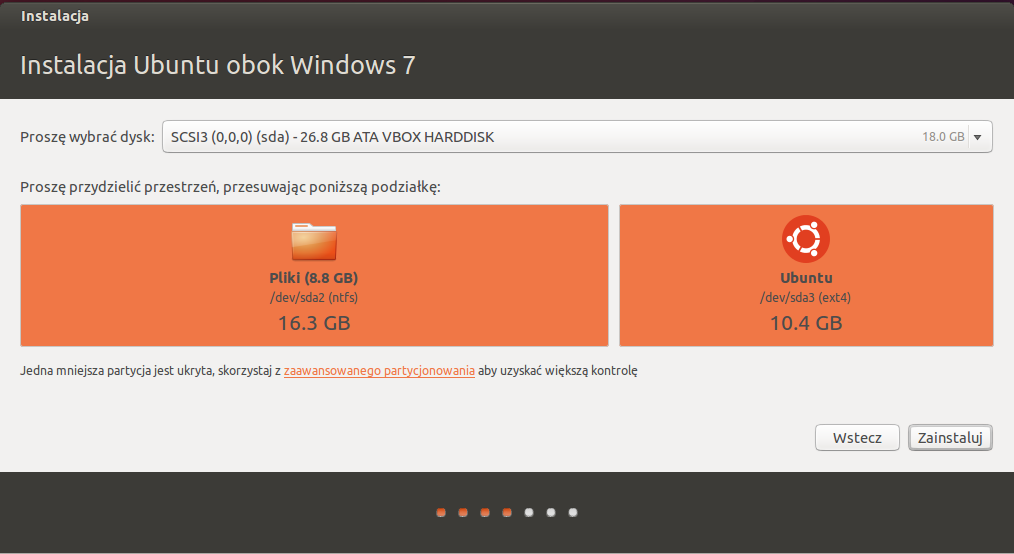
\includegraphics[scale=0.5]{images/instalator_partycjonowanie_obok_wondows7_2.png}]
\end{center}
Drugą możliwością jest instalacja Ubuntu obok już zainstalowanego systemu Windows. Jeżeli wybierzesz tę opcję to następny ekran pozwoli wybrać o ile instalator ma zmniejszyć partycję na której zainstalowany jest system Windows. Użyj myszy aby przesunąć pomarańczową podziałkę w lewo (więcej miejsca dla Ubuntu) lub w prawo(więcej miejsca dla Windowsa). Oryginalna partycja systemu Windows jest oznaczona na tym obrazie jako "Pliki". Pamiętaj, że ubuntu potrzebuje minimum 6,2 gigabajta przestrzeni, ale tak mała partycja zostanie prawie w całości wypełniona przez system i na Twoje pliki pozostanie niewiele miejsca.

\begin{flushright}
Kliknij na przycisk \textbf{Zainstaluj} aby przejść dalej.\\
Zostaniesz poproszony o potwierdzenie. Upewnij się, że wszystko jest w pożądku i kliknij \textbf{Naprzód}.\\
W tym momencie wybrane zmiany zostaną zapisane na dysku twardym.
\end{flushright}
\clearpage

\subsubsection{Szyfrowanie dysku twardego}
\begin{center}
	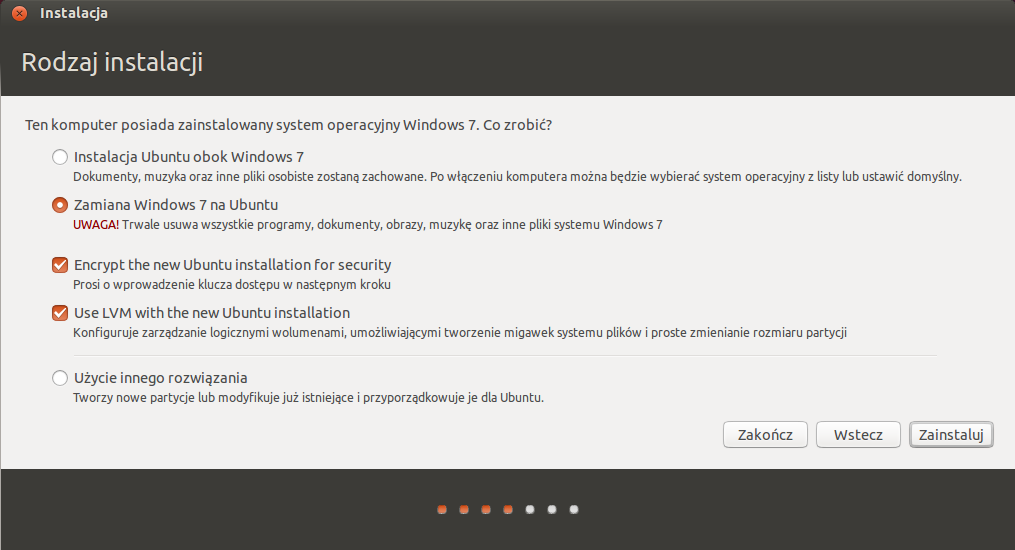
\includegraphics[scale=0.5]{images/instalator_partycjonowanie_szyfrowanie1.png}]
\end{center}
Przy wyborze jednego z automatycznych rozwiązań partycjonowania miałeś możliwości zastosowania szyfrowania dysku twardego. Wybranie tej opcji ukaże ci okno jak na powyższym obrazku. Zaszyfrowanie dysku twardego sprawie, że nikt nie uzyska dostępu do twoich danych ani nie zmodyfikuje zainstalowanego systemu. Wadą tego rozwiązania jest pewien narzut na procesor komputera i związane z tym zmniejszenie płynności działania komputera. Nowoczesne procesory zapewniają akcelerację sprzętową dla obliczeń kryptograficznych, w związku z czym utrata wydajności będzie się mieścić w granicach 5\% przy intensywnych opracacjach dyskowych.
\begin{flushright}
Kliknij na przycisk \textbf{Zainstaluj} aby przejść dalej.
\end{flushright}
\clearpage
\begin{center}
	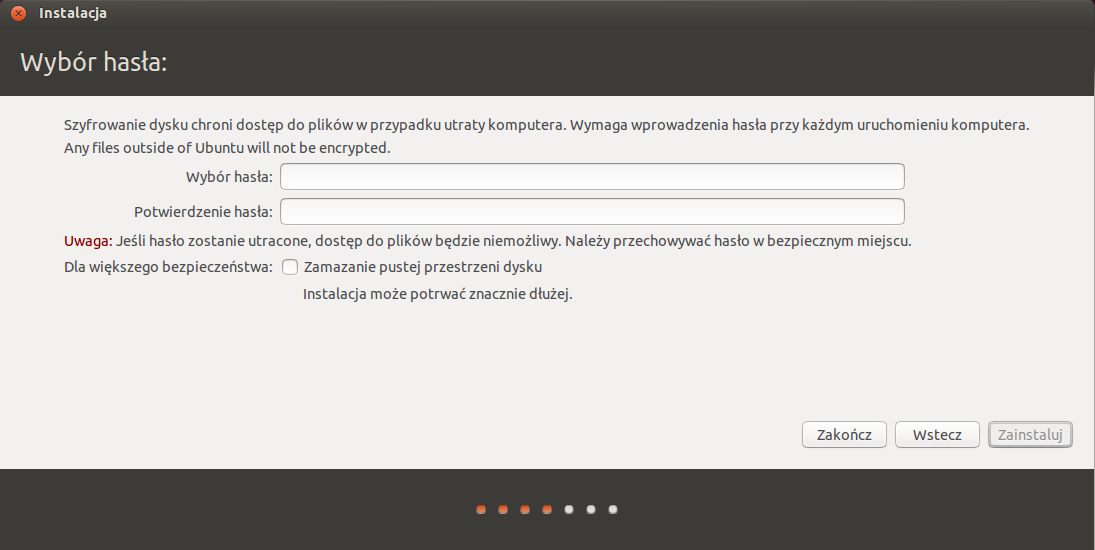
\includegraphics[scale=0.5]{images/instalator_partycjonowanie_szyfrowanie2.png}]
\end{center}
Na tym ekranie podaj hasło - klucz do dysku twardego. To nie jest to samo hasło, które ustawisz dla swojego systemowego konta a jedynie hasło umożliwiające dostęp do danych zapisanych na dysku twardym. Pamiętaj, że jeżeli zapomnisz hasła jakie zostanie tu wprowadzone, nie będzie możliwości odzyskania zaszyfrowanych danych. Postaraj się też aby hasło nie było łatwe do odgadnięcia, ale łatwe dla ciebie do zapamiętania.

Opcja "Zamazanie pustej przestrzeni dysku" powoduje, że niewykorzystywana, wolna przestrzeń dysku zostanie nadpisana losowymi danymi. Taka operacja znacznie utródnia potencjalnym włamywaczą włamanie się do twoich danych. Miej na uwadze, że zamazywanie pustej przestrzeni może trwać bardzo długo, w zależności do tego ile miejsca przeznaczysz na Ubuntu.

\begin{flushright}
Kliknij na przycisk \textbf{Zainstaluj} aby przejść dalej.\\
Zostaniesz poproszony o potwierdzenie. Upewnij się, że wszystko jest w pożądku i kliknij \textbf{Naprzód}
W tym momencie wybrane zmiany zostaną zapisane na dysku twardym.\\
\end{flushright}
\clearpage

\subsubsection{Zaawansowane partycjonowanie}
\begin{center}
	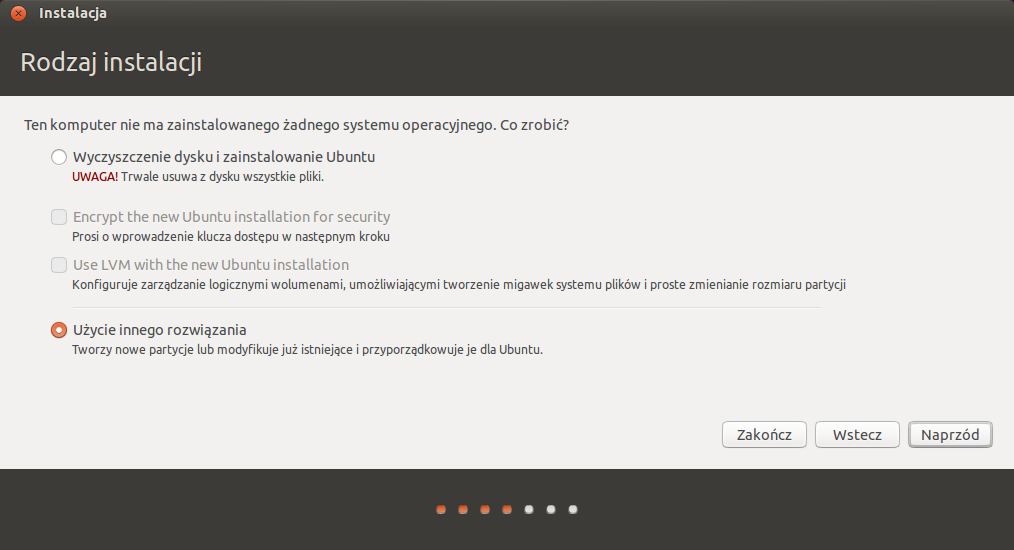
\includegraphics[scale=0.5]{images/instalator_partycjonowanie_gparted1.png}]
\end{center}
"Użycie innego rozwiązania" uruchamia program GParted, który umożliwia nieograniczone modyfikowanie partycji na dysku twardym. Jest to opcja dla bardziej zaawansowanych użytkowników, którzy mają świadomość tego jak działa partycjonowanie i jak powinien zostac podzielony ich dysk twardy. Jednak jeżeli na swoim komputerze maasz zainstalowany więcej niż jeden system operacyjny lub z jakiegoś innego powodu przedstawione wcześniej opcje nie spełniają twoich wymagań, to konieczne będzie sięgnięcie do zaawansowanego partycjonowania.

Do GParted warto zajrzeć jeszcze z jednego powodu. Podział partycji stosowany przez automatyczną instalację nie jest idealny. Ręczne ustawienie partycji da większa kontrolę i pozwoli znacznie lepiej dopasować układ partycji. 
\begin{flushright}
Kliknij na przycisk \textbf{Naprzód} aby przejść dalej.\\
\end{flushright}
\clearpage
%\begin{center}
%	\includegraphics[scale=0.5]{images/instalator_gparted2.png}]
%\end{center}
Na powyższym obrazku widzimy:
\begin{enumerate}
\item Menu wyboru dysku twardego. Jeżeli masz więcej niż jeden dysk twardy to tutaj go zmienisz.
\item Graficzna reprezentacja istniejącego rozkładu partycji na wybranym dysku twardym.
\item Przyciski dodawania i usówania partycji
\item Przycisk zmiany rozmiaru partycji
\item Informacje o aktualnie wybranej partycji
\end{enumerate}

\clearpage

\subsubsection{Zaawansowane partycjonowanie - instalacja na czystym dysku twardym}

\subsubsection{Zaawansowane partycjonowanie - instalacja obok innego systemu Linux}

\subsubsection{Zaawansowane partycjonowanie - Instalacja obok systemu Windows}

\subsubsection{Zaawansowane partycjonowanie - Instalacja z wykorzystaniem partycji utworzonej na systemie Windows 8}